\newpage
\section{Introduction}
\label{sec:introduction}

The objective of this laboratory assignment is to design and implement a BandPass Filter (BPF) with a central frequency of $1kHz$ and a gain at the central frequency of $40dB$.

Next, on table ~\ref{tab:restrictions} is the list of restrictions for this design:

\begin{table}[h]
    \centering
    \begin{tabular}{|l|c|}
    \hline
    {\bf Name} & {\bf Maximum Quantity} \\ \hline
    $741 OP-AMP$ & $1$ \\ \hline
    $1k{\Omega} Resistor$ & $3$ \\ \hline
    $10k{\Omega}Resistor$ & $3$ \\ \hline
    $100k{\Omega} Resistor$ & $3$ \\ \hline
    $220nf  capactior$ & $3$ \\ \hline
    $1{\mu}f  capacitor$ & $3$ \\ \hline
    \end{tabular}
    \caption{Restrictions for this assignment}
    \label{tab:restrictions}
\end{table}


\begin{figure}[!ht] \centering

\caption{Audio Amplifier Circuit}
\squeezeup
\squeezeup



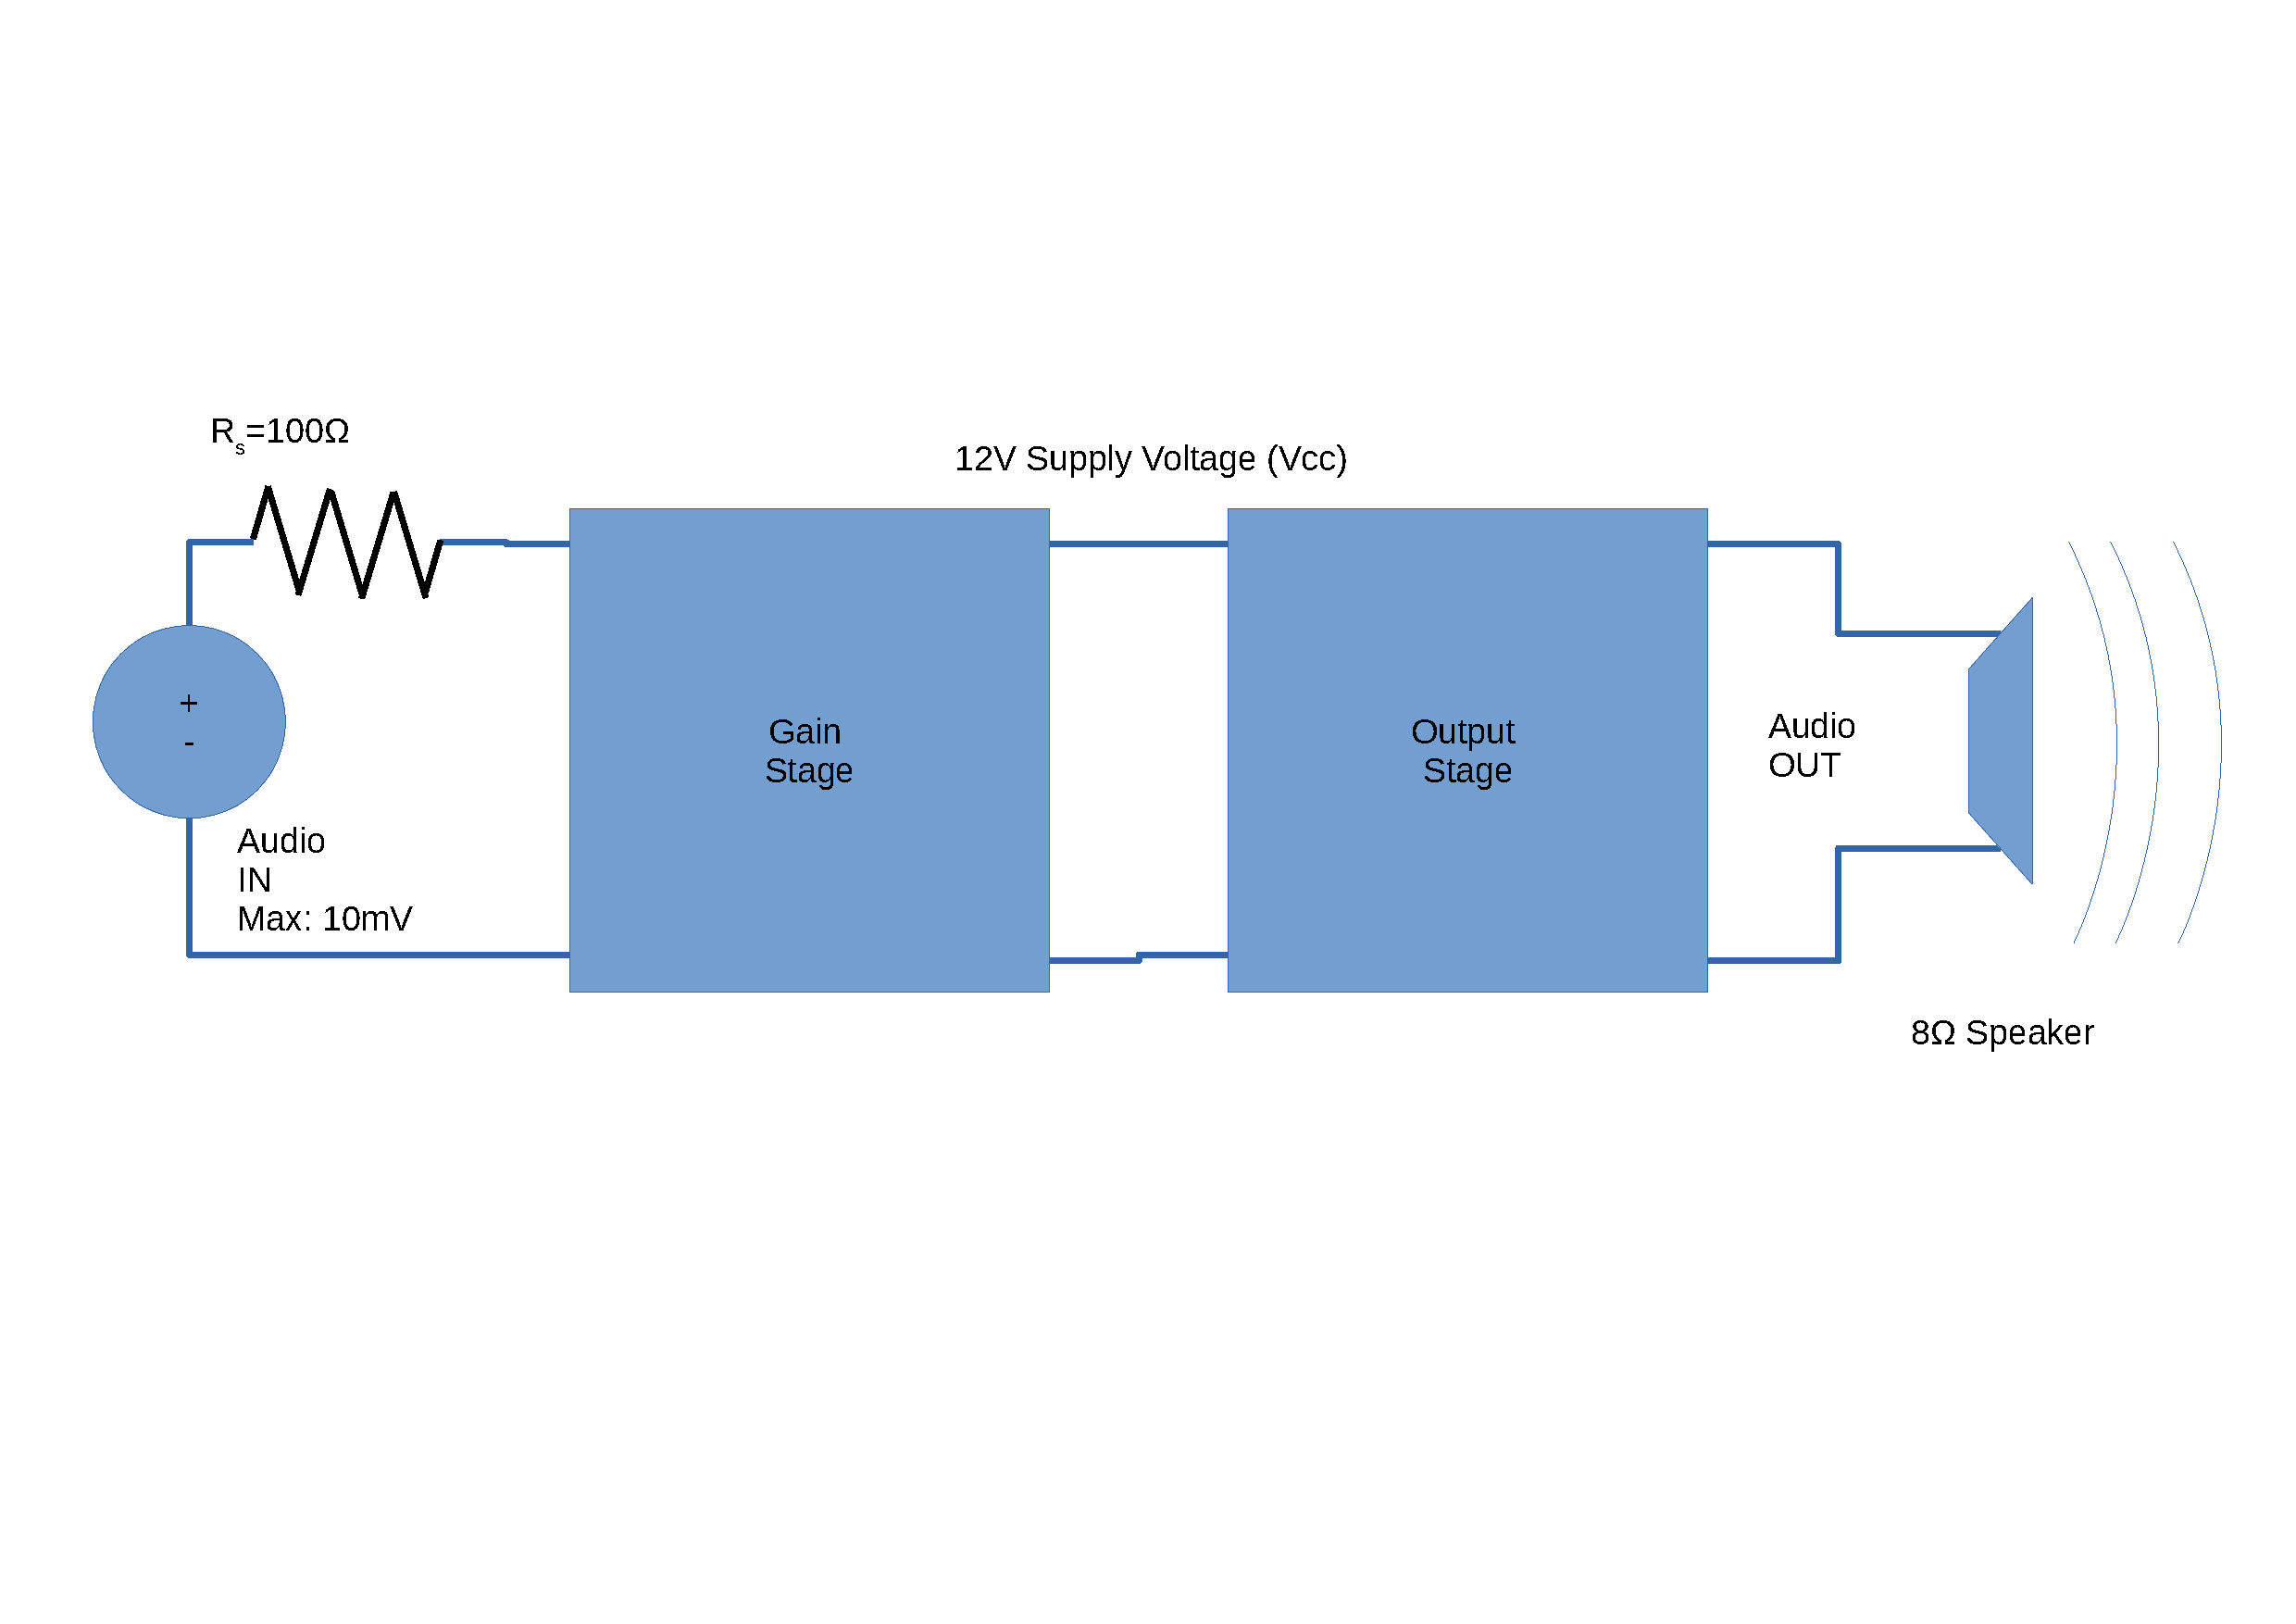
\includegraphics[width=1\textwidth, scale=1.0]{DesenhoT4.pdf}  
\squeezeup
\squeezeup
\squeezeup
\squeezeup
\squeezeup
\squeezeup
\label{fig:circuit}
\end{figure}

As mentioned above, it is also important to refer that we have developed an optimization algorithm (in Octave) in order to find the number of transistors, the values of the resistors and capacitor that would lead to the best value of merit, computed in Ngspice with the formula given by the Professor.   

